\chapter{Esercizi Prima Intercorso}



\begin{Esercizio1}
Dato l'insieme di task periodici in tabella, in cui, per 
ogni task si ipotizza l'uso di al massimo 4 sezioni critiche 
sui semafori $S_1$, $S_2$, $S_3$, ed $S_4$ ed in cui i valori 
nelle colonne $S_i$ rappresentano le durate massime 
delle rispettive sezioni critiche, si determini 
se l'insieme è schedulabile con RM e priority 
inheritance, utilizzando il test di Liu e Layland

\begin{table}[h]
\centering
\begin{tabular}{|c|c|c|c|c|c|c|}
\hline
\(\tau\) & $C_i$ & $T_i$ & $S_1$ & $S_2$ & $S_3$ & $S_4$ \\
\hline
$J_1$ & 15 & 70 & 2 & 4 & 5 & 0 \\
\hline
$J_2$ & 6 & 20 & 0 & 2 & 0 & 4 \\
\hline
$J_3$ & 10 & 135 & 1 & 3 & 0 & 5 \\
\hline
$J_4$ & 5 & 30 & 3 & 0 & 0 & 1 \\
\hline
\end{tabular}
\label{tab:task_periodici}
\end{table}




Ordiniamo i task in ordine di priorità:
\begin{table}[h]
\centering
\begin{tabular}{|c|c|c|c|c|c|c|}
\hline
\(\tau\) & $C_i$ & $T_i$ & $S_1$ & $S_2$ & $S_3$ & $S_4$ \\
\hline
$J_2$ & 6 & 20 & 0 & 2 & 0 & 4 \\
\hline
$J_4$ & 5 & 30 & 3 & 0 & 0 & 1 \\
\hline
$J_1$ & 15 & 70 & 2 & 4 & 5 & 0 \\
\hline
$J_3$ & 10 & 135 & 1 & 3 & 0 & 5 \\
\hline
\end{tabular}
\label{tab:task_periodici}
\end{table}





Calcoliamo i \(B_i\) per ogni task. Partiamo da \(B_2\),
ricordando che vale:
\begin{table}[h]
\centering
\begin{tabular}{|c|c|c|c|c|c|c|}
\hline
\(\tau\) & $C_i$ & $T_i$ & $S_1$ & $S_2$ & $S_3$ & $S_4$ \\
\hline
$J_2$ & 6 & 20 & 0 & 2 & 0 & 4 \\

\arrayrulecolor{red}\hline
\arrayrulecolor{black}

$J_4$ & 5 & 30 & 3 & 0 & 0 & 1 \\
\hline
$J_1$ & 15 & 70 & 2 & 4 & 5 & 0 \\
\hline
$J_3$ & 10 & 135 & 1 & 3 & 0 & 5 \\
\hline
\end{tabular}
\label{tab:task_periodici}
\end{table}

Selezioniamo solo i semafori con ceiling maggiore o uguale
alla priorità di \(J_{2}\), cioè i semafori \(S_{2}\) e \(S_{4}\):






\begin{table}[H]
\centering
\begin{tabular}{|c|c|c|c|c|c|c|}
\hline
\(\tau\) & $C_i$ & $T_i$ & $S_1$ &  \cellcolor{blue!20} $S_2$ & $S_3$ & \cellcolor{blue!20} $S_4$ \\
\hline
$J_2$ & 6 & 20 & 0 & 2 & 0 & 4 \\

\arrayrulecolor{red}\hline
\arrayrulecolor{black}

$J_4$ & 5 & 30 & 3 & 0 & 0 & 1 \\
\hline
$J_1$ & 15 & 70 & 2 & 4 & 5 & 0 \\
\hline
$J_3$ & 10 & 135 & 1 & 3 & 0 & 5 \\
\hline
\end{tabular}
\label{tab:task_periodici}
\end{table}


\begin{table}[H]
\centering
\begin{tabular}{|c|c|c|c|c|c|c|}
\hline
\(\tau\) & $C_i$ & $T_i$ & $S_1$ & $S_2$ & $S_3$ & $S_4$ \\
\hline
$J_2$ & 6 & 20 & 0 & 2 & 0 & 4 \\

\arrayrulecolor{red}\hline
\arrayrulecolor{black}

$J_4$ & 5 & 30 & 3 & \cellcolor{blue!20}0 & 0 & \cellcolor{blue!20}1 \\
\hline
$J_1$ & 15 & 70 & 2 & \cellcolor{blue!20}4 & 5 & \cellcolor{blue!20}0 \\
\hline
$J_3$ & 10 & 135 & 1 & \cellcolor{blue!20}3 & 0 & \cellcolor{blue!20}5 \\
\hline
\end{tabular}
\label{tab:task_periodici}
\end{table}





Ora selezioniamo di questi semafori solo le righe sotto la riga di \(J_{2}\):


\begin{table}[H]
\centering
\begin{tabular}{|c|c|c|c|c|c|c|}
\hline
\(\tau\) & $C_i$ & $T_i$ & $S_1$ &  \cellcolor{blue!20} $S_2$ & $S_3$ & \cellcolor{blue!20} $S_4$ \\
\hline
$J_2$ & 6 & 20 & 0 & 2 & 0 & 4 \\

\arrayrulecolor{red}\hline
\arrayrulecolor{black}

$J_4$ & 5 & 30 & 3 & 0 & 0 & 1 \\
\hline
$J_1$ & 15 & 70 & 2 & 4 & 5 & 0 \\
\hline
$J_3$ & 10 & 135 & 1 & 3 & 0 & 5 \\
\hline
\end{tabular}
\label{tab:task_periodici}
\end{table}


Ora calcoliamo \(B_{4}\):

\[B_{4}^{l} = 4 + 5 = 9 \]
\[B_{4}^{s} = 2 +4 +5= 11 \]

Dunque si ha che \(B_{4}\) vale:
\[ B_{4} = \min \left\{B_{4}^{l} , B_{4}^{s}\right\} =
 \min \left\{9 , 11\right\} = 9 \]

 Ora calcoliamo \(B_{1}\):
\[B_{1}^{l} = 5\]
\[B_{1}^{s} = 1 + 3 + 0 +5 = 9 \]
Dunque si ha che \(B_{1}\) vale:
\[ B_{1} = \min \left\{B_{1}^{l} , B_{1}^{s}\right\} =
 \min \left\{5 , 9\right\} = 5 \]

Infine \(B_{3}\) vale:
\[B_{3} = 0\]

Verifichiamo la schedulabilità con il test di Liu e Layland, che ricordiamo essere una condizione
solo sufficente.

Si ha che:
\[ \forall i, 1 \le i \le n, \sum_{k=1}^{i} \frac{C_{k}}{T_{k}} 
+ \frac{B_{i}}{T_{i}} \leq  i (2^{1/i} - 1) \]
In cui in questa formula i task dovrebbero essere ordinati in ordine di priorità,
con \(1\) il più prioritario ed \( n \) il meno prioritario.
Andiamo ad applicare la formula per ogni \(i\):
\[ J_{2} : \frac{C_{2}}{T_{2}} + \frac{B_{2}}{T_{2}} \leq 1 (2^{1/1} - 1) = 1 \]
\[J_{2} : \frac{6}{20} + \frac{9}{20} = \frac{15}{20}\leq 1 \]


\[ J_{4} : \frac{C_{2}}{T_{2}} + \frac{C_{4}}{T_{4}} + \frac{B_{4}}{T_{4}} \leq 2 (2^{1/2} - 1) = 0.828 \]
\[ J_{4} : \frac{6}{20} + \frac{5}{30} + \frac{9}{30} = 0.766 \leq  0.828 \]

\[ J_{1} : \frac{C_{2}}{T_{2}} + \frac{C_{4}}{T_{4}} + 
\frac{C_{1}}{T_{1}} + \frac{B_{1}}{T_{1}} \leq 3 (2^{1/3} - 1) = 0.7798 \]
\[ J_{1} : \frac{6}{20} + \frac{5}{30} + \frac{15}{70} + \frac{5}{70} = 0.7523 \leq 0.7798 \]


\[J_{3} : \frac{C_{2}}{T_{2}} + \frac{C_{4}}{T_{4}} + 
\frac{C_{1}}{T_{1}} +
 \frac{C_{3}}{T_{3}} + \frac{B_{3}}{T_{3}} \leq 4 (2^{1/4} - 1) = 0.7568 \]
\[J_{3} : \frac{6}{20} + \frac{5}{30} + \frac{15}{70} + 
\frac{10}{135} = 0.7550 \leq 0.7568 \
 \]

 Dunque l'insieme di task è schedulabile con RM e priority inheritance.

\end{Esercizio1}


\begin{Esercizio2}

Consideriamo i seguenti task periodici:

\begin{table}[h]
\centering
\begin{tabular}{|c|c|c|c|c|c|c|c|}
\hline
\(\tau\) & $C_i$ & $T_i$ & $S_1$ & $S_2$ & $S_3$ & $S_4$ & $S_5$ \\
\hline
$J_1$ & 5 & 28 & 0 & 0 & 2 & 1 & 0 \\
\hline
$J_2$ & 3 & 16 & 1 & 0 & 0 & 2 & 0 \\
\hline
$J_3$ & 4 & 60 & 1 & 0 & 2 & 3 & 0 \\
\hline
$J_4$ & 10 & 40 & 3 & 4 & 0 & 0 & 1 \\
\hline
$J_5$ & 10 & 100 & 0 & 2 & 1 & 0 & 4 \\
\hline
\end{tabular}
\label{tab:task_periodici_esercizio}
\end{table}

Per prima cosa bisogna riscrivere i task in ordine di priorità,
in cui un task con periodo minore (quindi con deadline minore)
ha priorità maggiore rispetto ad un task con periodo maggiore.
Dunque la nuova tabella diventa:

\begin{table}[h]
\centering
\caption{Task ordinati per priorità}
\begin{tabular}{|c|c|c|c|c|c|c|c|}
\hline
\(\tau\) & $C_i$ & $T_i$ & $S_1$ & $S_2$ & $S_3$ & $S_4$ & $S_5$ \\
\hline
$J_2$ & 3 & 16 & 1 & 0 & 0 & 2 & 0 \\
\hline
$J_1$ & 5 & 28 & 0 & 0 & 2 & 1 & 0 \\
\hline
$J_4$ & 10 & 40 & 3 & 4 & 0 & 0 & 1 \\
\hline
$J_3$ & 4 & 60 & 1 & 0 & 2 & 3 & 0 \\
\hline
$J_5$ & 10 & 100 & 0 & 2 & 1 & 0 & 4 \\
\hline
\end{tabular}
\label{tab:task_periodici_esercizio}
\end{table}

Calcoliamo i \(B_i\). Partiamo da \(B_2\),
ricordando che vale:
\[ B_2 = \min \left\{B_{1}^{l} , B_{2}^{s}\right\} \]
Calcoliamo \(B_{1}^{l}\).
Notiamo per prima cosa che \(C(J_{2}) = P_{2}\),
andiamo quindi a selezionare solo i semafori 
con \(C(S_{i}) \ge P_{2}\), cioè \(S_1\) e \(S_4\).
Per vederlo graficamente dobbiamo selezionare solo 
i semafori che hanno almeno un elemento diverso da 0 
sopra la linea rossa orizzontale che rappresenta la priorità
\(J_{2}\):

\begin{table}[h]
\centering
\caption{Task ordinati per priorità}
\begin{tabular}{|c|c|c|c|c|c|c|c|}
\hline
\(\tau\) & $C_i$ & $T_i$ & $S_1$ & $S_2$ & $S_3$ & $S_4$ & $S_5$ \\
\hline
$J_2$ & 3 & 16 & 1 & 0 & 0 & 2 & 0 \\
\arrayrulecolor{red}\hline
\arrayrulecolor{black}
$J_1$ & 5 & 28 & 0 & 0 & 2 & 1 & 0 \\
\hline
$J_4$ & 10 & 40 & 3 & 4 & 0 & 0 & 1 \\
\hline
$J_3$ & 4 & 60 & 1 & 0 & 2 & 3 & 0 \\
\hline
$J_5$ & 10 & 100 & 0 & 2 & 1 & 0 & 4 \\
\hline
\end{tabular}
\label{tab:task_periodici_esercizio}
\end{table}

Dunque i semafori che hanno almeno un elemento diverso da 
0 sono \(S_{1}\) e \(S_{4}\):


\begin{table}[h]
\centering
\begin{tabular}{|c|c|c|c|c|c|c|c|}
\hline
\(\tau\) & $C_i$ & $T_i$ & \cellcolor{blue!20}$S_1$ & $S_2$ & $S_3$ & \cellcolor{blue!20}$S_4$ & $S_5$ \\
\hline
$J_2$ & 3 & 16 & \cellcolor{blue!20}1 & 0 & 0 & \cellcolor{blue!20}2 & 0 \\
\arrayrulecolor{red}\hline
\arrayrulecolor{black}
$J_1$ & 5 & 28 & \cellcolor{blue!20}0 & 0 & 2 & \cellcolor{blue!20}1 & 0 \\
\hline
$J_4$ & 10 & 40 & \cellcolor{blue!20}3 & 4 & 0 & \cellcolor{blue!20}0 & 1 \\
\hline
$J_3$ & 4 & 60 & \cellcolor{blue!20}1 & 0 & 2 & \cellcolor{blue!20}3 & 0 \\
\hline
$J_5$ & 10 & 100 & \cellcolor{blue!20}0 & 2 & 1 & \cellcolor{blue!20}0 & 4 \\
\hline
\end{tabular}
\label{tab:task_periodici_esercizio}
\end{table}

Ora andiamo a selezionare di questi semafori solo le 
righe sono la riga di \(J_{2}\):


\begin{table}[H]
\centering
\caption{Task ordinati per priorità}
\begin{tabular}{|c|c|c|c|c|c|c|c|}
\hline
\(\tau\) & $C_i$ & $T_i$ & $S_1$ & $S_2$ & $S_3$ & $S_4$ & $S_5$ \\
\hline
$J_2$ & 3 & 16 & 1 & 0 & 0 & 2 & 0 \\
\arrayrulecolor{red}\hline
\arrayrulecolor{black}
$J_1$ & 5 & 28 & \cellcolor{blue!20}0 & 0 & 2 & \cellcolor{blue!20}1 & 0 \\
\hline
$J_4$ & 10 & 40 & \cellcolor{blue!20}3 & 4 & 0 & \cellcolor{blue!20}0 & 1 \\
\hline
$J_3$ & 4 & 60 & \cellcolor{blue!20}1 & 0 & 2 & \cellcolor{blue!20}3 & 0 \\
\hline
$J_5$ & 10 & 100 & \cellcolor{blue!20}0 & 2 & 1 & \cellcolor{blue!20}0 & 4 \\
\hline
\end{tabular}
\label{tab:task_periodici_esercizio}
\end{table} 

Ora per calcolare \(B_{2}^{l}\) per ogni riga sotto 
\(J_{2}\) andiamo 
a fare il massimo solo tra gli elementi delle colonne
dei semafori selezionati, cioè \(S_{1}\) e \(S_{4}\):


\begin{table}[H]
\centering
\begin{tabular}{|c|c|c|c|c|c|c|c|c|}
\hline
\(\tau\) & $C_i$ & $T_i$ & $S_1$ & $S_2$ & $S_3$ & $S_4$ & $S_5$ & $\max$ \\
\hline
$J_2$ & 3 & 16 & 1 & 0 & 0 & 2 & 0 & \\
\arrayrulecolor{red}\hline
\arrayrulecolor{black}
$J_1$ & 5 & 28 & \cellcolor{blue!20}0 & 0 & 2 & \cellcolor{blue!20}1 & 0 & 1 \\
\hline
$J_4$ & 10 & 40 & \cellcolor{blue!20}3 & 4 & 0 & \cellcolor{blue!20}0 & 1 & 3 \\
\hline
$J_3$ & 4 & 60 & \cellcolor{blue!20}1 & 0 & 2 & \cellcolor{blue!20}3 & 0 & 3 \\
\hline
$J_5$ & 10 & 100 & \cellcolor{blue!20}0 & 2 & 1 & \cellcolor{blue!20}0 & 4 & 0 \\
\hline
\end{tabular}
\label{tab:task_periodici_esercizio}
\caption{Massimi per calcolo \(B_{i}^{l}\)}

\end{table}

\(B_{2}^{l}\) è dato dalla somma dei massimi:
\[ B_{2}^{l} = 1 + 3 + 3 + 0 = 7 \]




Ora calcoliamo \(B_{2}^{s}\). Per calcolarlo dobbiamo
considerare come prima tutti i semafori per cui si ha 
\(C(S_{i}) \ge P_{2}\), che come prima sono solo
 \(S_{1}\) e \(S_{4}\). Di questi semafori 
 consideriamo solo le righe che stanno sotto \(J_{2}\):


\begin{table}[H]
\centering
\begin{tabular}{|c|c|c|c|c|c|c|c|}
\hline
\(\tau\) & $C_i$ & $T_i$ & $S_1$ & $S_2$ & $S_3$ & $S_4$ & $S_5$ \\
\hline
$J_2$ & 3 & 16 & 1 & 0 & 0 &2 & 0 \\
\arrayrulecolor{red}\hline
\arrayrulecolor{black}
$J_1$ & 5 & 28 & \cellcolor{blue!20}0 & 0 & 2 & \cellcolor{blue!20}1 & 0 \\
\hline
$J_4$ & 10 & 40 & \cellcolor{blue!20}3 & 4 & 0 & \cellcolor{blue!20}0 & 1 \\
\hline
$J_3$ & 4 & 60 & \cellcolor{blue!20}1 & 0 & 2 & \cellcolor{blue!20}3 & 0 \\
\hline
$J_5$ & 10 & 100 & \cellcolor{blue!20}0 & 2 & 1 & \cellcolor{blue!20}0 & 4 \\
\hline
\end{tabular}
\label{tab:task_periodici_esercizio}
\end{table}
Ora per ogni semaforo selezionato (dunque per ogni colonna
selezionata)
andiamo a fare il massimo tra gli elementi del semaforo
(aggiungiamo una riga per fare vedere i massimi):


\begin{table}[H]
\centering
\begin{tabular}{|c|c|c|c|c|c|c|c|}
\hline
\(\tau\) & $C_i$ & $T_i$ & $S_1$ & $S_2$ & $S_3$ & $S_4$ & $S_5$ \\
\hline
$J_2$ & 3 & 16 & 1 & 0 & 0 & 2 & 0 \\
\arrayrulecolor{red}\hline
\arrayrulecolor{black}
$J_1$ & 5 & 28 & \cellcolor{blue!20}0 & 0 & 2 & \cellcolor{blue!20}1 & 0 \\
\hline
$J_4$ & 10 & 40 & \cellcolor{blue!20}3 & 4 & 0 & \cellcolor{blue!20}0 & 1 \\
\hline
$J_3$ & 4 & 60 & \cellcolor{blue!20}1 & 0 & 2 & \cellcolor{blue!20}3 & 0 \\
\hline
$J_5$ & 10 & 100 & \cellcolor{blue!20}0 & 2 & 1 & \cellcolor{blue!20}0 & 4 \\
\hline
max & & & 3 & & & 3 & \\
\hline
\end{tabular}
\label{tab:task_periodici_esercizio}
\end{table}

\(B_{2}^{s}\) è dato dalla somma dei massimi:
\[ B_{2}^{s} = 3 + 3 = 6 \]

Dunque \(B_{2}\) sarà:
\[ B_{2} = \min \left\{B_{2}^{l} , B_{2}^{s}\right\} =
 \min \left\{7 , 6\right\} = 6 \]

\end{Esercizio2}




\begin{Esercizio3}

Dato l'insieme di task in tabella, in cui, 
per ogni task si riporta la richiesta
 di utilizzo massima di 4 risorse R1, R2, R3, ed 
 R4 disponibili in un massimo di 4, 2, 3 e 1 unità, 
 si calcoli il ceiling \(C_{R}(n_{R})\) per tutte e tre le risorse, 
 al variare del numero di risorse disponibili. 
 Nel caso in cui siano correttamente disponibili 3
  unità di R1, 1 unità di R2, 0 unità di R3 e 1 
  unità di R4, quale sarà il valore assunto dal 
  ceiling del sistema \(\pi_{S}\)?

  \begin{table}[H]
\centering
\begin{tabular}{|c|c|c|c|c|c|}
\hline
& $D_i$ & $\mu_{R1}$ & $\mu_{R2}$ & $\mu_{R3}$ & $\mu_{R4}$ \\
\hline
$J_1$ & 35 & 4 & 1 & 0 & 1 \\
\hline
$J_2$ & 10 & 3 & 1 & 0 & 0 \\
\hline
$J_3$ & 140 & 2 & 0 & 3 & 1 \\
\hline
$J_4$ & 80 & 1 & 2 & 2 & 0 \\
\hline
\end{tabular}
\caption{Richieste di task e disponibilità di risorse}
\end{table}

Odiniamo i task in ordine di priorità:

  \begin{table}[H]
\centering
\begin{tabular}{|c|c|c|c|c|c|}
\hline
& $D_i$ & $\mu_{R1}$ & $\mu_{R2}$ & $\mu_{R3}$ & $\mu_{R4}$ \\
\hline
$J_2$ & 10 & 3 & 1 & 0 & 0 \\
\hline
$J_1$ & 35 & 4 & 1 & 0 & 1 \\
\hline
$J_4$ & 80 & 1 & 2 & 2 & 0 \\
\hline
$J_3$ & 140 & 2 & 0 & 3 & 1 \\

\hline
\end{tabular}
\caption{Task ordinati per priorità}
\end{table}


Assegniamo i livelli di preemption ai task in base alla loro priorità:

\begin{table}[H]
\centering
\begin{tabular}{|c|c|c|c|c|c|c|}
\hline
& $D_i$ & \(\pi_{i}\) & $\mu_{R1}$ & $\mu_{R2}$ & $\mu_{R3}$ & $\mu_{R4}$ \\
\hline
$J_2$ & 10 & 4 & 3 & 1 & 0 & 0 \\
\hline
$J_1$ & 35 & 3 & 4 & 1 & 0 & 1 \\
\hline
$J_4$ & 80 & 2 & 1 & 2 & 2 & 0 \\
\hline
$J_3$ & 140 & 1 & 2 & 0 & 3 & 1 \\

\hline
\end{tabular}
\caption{Task ordinati per priorità}
\end{table}


\begin{table}[H]
\centering
\begin{tabular}{|c|c|}
\hline
\(R_{i}\) & \(U_{i}\) \\
\hline
\(R_{1}\) & 4 \\
\hline
\(R_{2}\) & 2 \\
\hline
\(R_{3}\) & 3 \\
\hline
\(R_{4}\) & 1 \\
\hline
\end{tabular}
\end{table}


Costruiamo ora la tabella dei ceiling delle risorse:

\begin{table}[H]
\centering  
\begin{tabular}{|c|c|c|c|c|c|}
\hline
& 4 & 3& 2 & 1 & 0\\
\hline
$R_1$ & 0 & 3 & 4 & 4 & 4\\
\hline
$R_2$ & - & - & 0 & 2 & 4\\
\hline
$R_3$ & - & 0 & 1 & 2 & 2\\
\hline
$R_4$ & - & - & - & 0 &  3\\
\hline
\end{tabular}
\caption{Ceiling delle risorse}
\end{table}

Il ceiling di sistema \(\pi_{S}\) quando si hanno 3 unità di R1, 1 unità di R2,
0 unità di R3 e 1 unità di R4 è dato da:
\[\pi_{S} = \max \{ \textcolor{red}{C_{R1}(3)}, 
\textcolor{blue}{C_{R2}(1)}, \textcolor{green}{C_{R3}(0)}, 
\textcolor{violet}{ C_{R4}(1)} \} = \max \{
\textcolor{red}{3}, \textcolor{blue}{2}, \textcolor{green}{2}, \textcolor{violet}{0}\} = 4 \]


\begin{table}[H]
\centering  
\begin{tabular}{|c|c|c|c|c|c|}
\hline
& 4 & 3& 2 & 1 & 0\\
\hline
$R_1$ & 0 & \textcolor{red}{3} & 4 & 4 & 4\\
\hline
$R_2$ & - & - & 0 & \textcolor{blue}{2} & 4\\
\hline
$R_3$ & - & 0 & 1 & 2 & \textcolor{green}{2}\\
\hline
$R_4$ & - & - & - & \textcolor{violet}{0} &  3\\
\hline
\end{tabular}
\caption{Ceiling delle risorse}
\end{table}
\end{Esercizio3}


\begin{Esercizio4}

Dato l'insieme di task periodici in tabella, in cui, per ogni task si ipotizza 
l'uso di al massimo 4 sezioni critiche sui semafori $S_1$, $S_2$, $S_3$, ed $S_4$ 
ed in cui i valori nelle colonne $S_i$ rappresentano le durate massime delle 
rispettive sezioni critiche, si determini se l'insieme è schedulabile con EDF 
e Stack Resource Policy (SRP) con il test di Liu e Layland, assumendo che i task 
con periodo minore abbiano maggior livello di preemption. I tempi di bloccaggio 
possono essere calcolati con il metodo che si adotta per il priority ceiling.

\begin{table}[H]
\centering
\begin{tabular}{|c|c|c|c|c|c|c|}
\hline
G & $T_i$ & $C_i$ & $S_1$ & $S_2$ & $S_3$ & $S_4$ \\
\hline
$J_1$ & 5 & 25 & 4 & 0 & 0 & 0 \\
\hline
$J_2$ & 12 & 150 & 0 & 5 & 0 & 6 \\
\hline
$J_3$ & 4 & 16 & 0 & 2 & 0 & 0 \\
\hline
$J_4$ & 2 & 10 & 0 & 0 & 1 & 0 \\
\hline
$J_5$ & 16 & 60 & 4 & 0 & 3 & 8 \\
\hline
\end{tabular}
\label{tab:task_esercizio3}
\end{table}


\end{Esercizio4}



\begin{Esercizio5}

Si considerino i task periodici indicati in tabella, con deadline relativa inferiore 
al periodo. Ciascun task utilizza al massimo di 2 risorse critiche protette 
rispettivamente dai semafori $S_1$ ed $S_2$ per i quali si riporta la durata massima 
delle sezioni critiche per ogni task. Supponendo che i task siano schedulati con 
algoritmo EDF e le risorse gestite con SRP, si verifichi la fattibilità dell'insieme 
dei task adottando il metodo del \textit{processor demand criterion}. Il calcolo dei 
tempi di bloccaggio può essere fatto con lo stesso metodo che si utilizza per il 
protocollo di priority ceiling.

\begin{table}[H]
\centering
\begin{tabular}{|c|c|c|c|c|c|}
\hline
$\tau$ & $C_i$ & $D_i$ & $T_i$ & $S_1$ & $S_2$ \\
\hline
$\tau_1$ & 4 & 6 & 20 & 0 & 0 \\
\hline
$\tau_2$ & 1 & 3 & 4 & 1 & 0 \\
\hline
$\tau_3$ & 2 & 8 & 10 & 0 & 2 \\
\hline
$\tau_4$ & 1 & 7 & 8 & 1 & 1 \\
\hline
\end{tabular}
\label{tab:task_edf_srp}
\end{table}

\end{Esercizio5}



\begin{Esercizio6}

\begin{table}[H]
\centering
\caption{Dati dei task (frequenza di attivazione e tempo di calcolo)}
\begin{tabular}{|c|c|c|c|c|c|}
\hline
 & $T_1$ & $T_2$ & $T_3$ & $T_4$ & $T_5$ \\
\hline
$f$ (Hz) & 25 & 100 & 12,5 & 6,25 & 50 \\
\hline
$C_i$ (ms) & 3 & 2 & 4 & 7 & 6 \\
\hline
\end{tabular}
\label{tab:timeline_tasks}
\end{table}

\noindent
Si consideri l'insieme di task periodici caratterizzati dalla frequenza di attivazione
(in Hz) e dal tempo di calcolo (in ms), riportati nella tabella precedente.
Ipotizzando l'uso del Timeline Scheduling (Cyclic Executive), si calcolino
il minor cycle (o time slot) e il major cycle (o iperperiodo) e si riporti
graficamente la schedulazione ottenuta allocando opportunamente le istanze
dei task nei time slot, ipotizzando che non vi siano vincoli sul jitter 
di attivazione dei job. Si riportino (e testino) anche le condizioni da 
verificare per assicurare la schedulabilità dei task nei time slot. Si ipotizzi
infine che il tempo di calcolo del task $T_5$ passi da 6 ms a 9 ms, rendendo la
schedulazione non fattibile: quale soluzione adottare in questo caso? Discutere
la possibile soluzione mostrando graficamente come si modifica la timeline e
riportando le nuove condizioni da verificare.


\end{Esercizio6}


\begin{Esercizio7}

Si consideri l'insieme di task periodici rappresentato nella tabella.  
Si determini se l'insieme è schedulabile con EDF mediante il test di Liu e Layland.  
Si ripeta poi il test attraverso il processor demand criterion, 
rappresentando graficamente la domanda di calcolo nell'iperperiodo
al variare del tempo $L$, e verificando che essa sia sempre inferiore 
alla funzione identità $g(L)=L$.

\begin{table}[H]
\centering
\caption{Dati dei task}
\begin{tabular}{|c|c|c|c|}
\hline
 & $\tau_1$ & $\tau_2$ & $\tau_3$ \\
\hline
$C_i$ & 2 & 3 & 6 \\
\hline
$D_i$ & 5 & 9 & 13 \\
\hline
$T_i$ & 6 & 12 & 18 \\
\hline
\end{tabular}
\label{tab:edf_tasks}
\end{table}


\[ 
\sum_{i=1}^{n} \frac{C_{i}}{D_{i}} \le n (2^{1/n} - 1)
\]
\[ \frac{C_{1}}{D_{1}} + \frac{C_{2}}{D_{2}} + \frac{C_{3}}{D_{3}} \le 3 (2^{1/3} - 1) \]
\[ \frac{2}{5} + \frac{3}{9} + \frac{6}{13} = 1.194 \ge 0.7798 \]
Dunque il test di Liu e Layland non è superato, ma esso è solo un test sufficiente,
quindi procediamo con il processor demand criterion.

Calcoliamo \(U\):
\[
\sum_{i=1}^{n} \frac{C_{i}}{T_{i}} = \frac{2}{6} + \frac{3}{12} + \frac{6}{18} = 0.9166  
\]
Calcoliamo \(L^{*}\):
\[
L^{*} = \frac{1}{1-U}\sum_{i=1}^{n} (T_{i} - D_{i}) U_{i} 
\]
In cui \(U_{i} = \displaystyle \frac{C_{i}}{T_{i}}\), dunque:
\[
L^{*} = \frac{1}{1-0.9166} 
\left( (6-5) \frac{2}{6} + (12-9) \frac{3}{12} + (18-13) \frac{6}{18} \right) = 32.97
\]

Calcoliamo l'iperperiodo:
\[ H = m.c.m.(6, 12, 18) = 36 \]


z<
\begin{figure}[h]
\centering
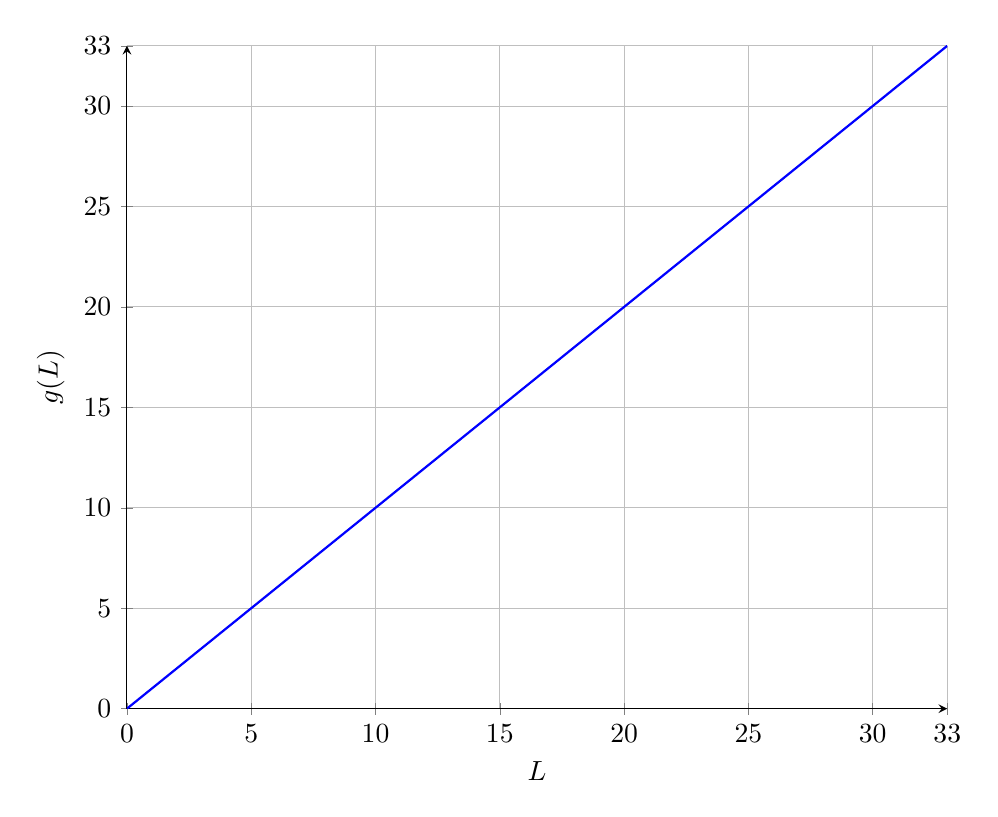
\begin{tikzpicture}
  \begin{axis}[
    axis lines=left,
    xmin=0, ymin=0, xmax=33, ymax=33,
    xlabel={$L$}, ylabel={$g(L)$},
    xtick={0,5,10,15,20,25,30,33},
    ytick={0,5,10,15,20,25,30,33},
    grid=both,
    width=12cm, height=10cm,
    domain=0:33,
    clip=true,
    enlargelimits=false,
  ]
    \addplot[blue, thick] {x}; % g(L) = L (linea identità)
  \end{axis}
\end{tikzpicture}
\end{figure}

\end{Esercizio7}


\begin{Esercizio8}







\end{Esercizio8}

\begin{Esercizio9}

  

Si consideri l'insieme di task periodici in tabella, 
con deadline $D_i$ minore del periodo $T_i$. 
Si determini se l'insieme è schedulabile con 
Deadline Monotonic (DM) attraverso il test di Liu e Layland. 
Si ripeta poi il test attraverso il metodo dell'interferenza $I_i$ e 
si discutano le differenze rispetto al test precedente, ove presenti.

\begin{table}[H]
\centering
\caption{Dati dei task}
\begin{tabular}{|c|c|c|c|c|c|}
\hline
 & $\tau_1$ & $\tau_2$ & $\tau_3$ & $\tau_4$ & $\tau_5$ \\
\hline
$C_i$ & 2 & 3 & 1 & 5 & 2 \\
\hline
$D_i$ & 11 & 15 & 8 & 37 & 10 \\
\hline
$T_i$ & 11 & 18 & 9 & 40 & 12 \\
\hline
\end{tabular}
\label{tab:dm_tasks}
\end{table}


Eseguiamo per prima cosa il test di Liu e Layland per DM:
\[
\sum_{i=1}^{n} \frac{C_{i}}{D_{i}} \le n (2^{1/n} - 1)
\]

\[\frac{2}{11} + \frac{3}{15} + \frac{1}{8} + \frac{5}{37} + \frac{2}{10} 
= 0.841
\ge 5 (2^{1/5} - 1) = 0.7435\]
Il test non è superato, ma ricordiamo che esso è solo un test sufficiente.



L'ordine di priorità dei task è:
\[
\tau_{3} > \tau_{5} > \tau_{1} > \tau_{2} > \tau_{4}
\]



Calcoliamo l'interferenza per ogni task:
\[ I_{3} = 0 \]
\[ I_{5} = \left \lceil \frac{D_{5}}{T_{3}} \right \rceil C_{3} = \left \lceil \frac{10}{9} \right \rceil  \cdot 1 = 2 \]
\[I_{1} = \left \lceil \frac{D_{1}}{T_{5}} \right \rceil C_{5}  + \left \lceil \frac{D_{1}}{T_{3}} \right \rceil C_{3}
=    \]

\[I_{2} = \left \lceil \frac{D_{2}}{T_{1}} \right \rceil C_{1} + \left \lceil \frac{D_{2}}{T_{5}} \right \rceil C_{5} 
 + \left \lceil \frac{D_{2}}{T_{3}} \right \rceil C_{3}
=   \]
\[I_{4} = \left \lceil \frac{D_{4}}{T_{2}} \right \rceil C_{2}  + 
\left \lceil \frac{D_{4}}{T_{1}} \right \rceil C_{1} + \left \lceil \frac{D_{4}}{T_{5}} \right \rceil C_{5} 
 + \left \lceil \frac{D_{4}}{T_{3}} \right \rceil C_{3}
=   \]


\end{Esercizio9}